% Compile with: xelatex main.tex (twice).
% Theme: metropolis (installed under /usr/share/texlive/texmf-dist/tex/latex/beamertheme-metropolis).
\documentclass[aspectratio=169,10pt]{beamer}

\usetheme{metropolis}
\metroset{numbering=fraction,progressbar=foot}

\usepackage{amsmath,amssymb}
\usepackage{braket}
\usepackage{physics}
\usepackage{tikz}
\usetikzlibrary{positioning,arrows.meta,decorations.pathreplacing,decorations.pathmorphing,fit,backgrounds}
\usepackage{booktabs}
\usepackage{xcolor}

\definecolor{e0col}{HTML}{1F77B4}
\definecolor{e1col}{HTML}{D62728}
\definecolor{midcol}{HTML}{6F42C1}

\title{Bell-State Preparation on a Two-Legged Ladder QPU}
\subtitle{Dynamic swap, and unitary GHZ-uncompute}
\date{2026 NCCU Applied Physics Challenge --- 14 May 2026}
\author{Overnight Research Company}

\begin{document}

\maketitle

% ============================================================
% Slide 2 — The challenge
% ============================================================
\begin{frame}{The challenge}
  \begin{columns}[T,onlytextwidth]
    \begin{column}{0.42\textwidth}
      \textbf{Goal.} Prepare a Bell state
      \[
        \ket{\Phi^+}_{e_0 e_1}
          = \tfrac{1}{\sqrt{2}}\bigl(\ket{00}+\ket{11}\bigr)
      \]
      between the two \emph{far-end} qubits of a two-legged ladder QPU,
      for any ladder length~$L$.
      \medskip

      \textbf{Constraints.}
      \begin{itemize}\setlength{\itemsep}{0.2em}
        \item Only nearest-neighbour gates (ladder edges).
        \item Top leg, bottom leg, rungs all allowed.
        \item Must scale to arbitrary $L$.
      \end{itemize}
    \end{column}
    \begin{column}{0.58\textwidth}
      \centering
      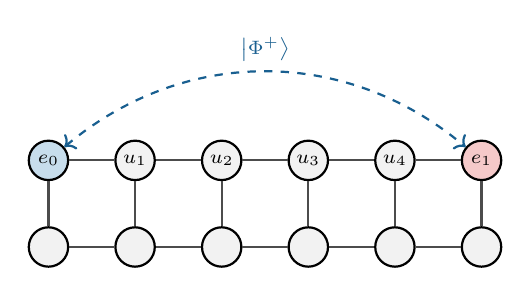
\begin{tikzpicture}[
          qubit/.style={circle,draw,thick,minimum size=5mm,inner sep=0pt,fill=white,font=\scriptsize},
          end/.style={qubit,fill=e0col!25},
          end2/.style={qubit,fill=e1col!25},
          inner/.style={qubit,fill=black!5},
          link/.style={thick,draw=black!70},
          x=11mm,y=11mm
        ]
        % Top leg
        \node[end] (e0) at (0,1) {$e_0$};
        \foreach \i in {1,2,3,4} {\node[inner] (u\i) at (\i,1) {$u_\i$};}
        \node[end2] (e1) at (5,1) {$e_1$};
        % Bottom leg
        \foreach \i in {0,1,2,3,4,5} {\node[inner] (b\i) at (\i,0) {};}
        % Top-leg edges
        \draw[link] (e0)--(u1)--(u2)--(u3)--(u4)--(e1);
        % Bottom-leg edges
        \draw[link] (b0)--(b1)--(b2)--(b3)--(b4)--(b5);
        % Rungs
        \foreach \i/\j in {0/e0,1/u1,2/u2,3/u3,4/u4,5/e1}
          {\draw[link] (b\i)--(\j);}
        % Target arrow
        \draw[<->,thick,e0col!80!black,dashed] (e0) to[bend left=40] node[midway,above,font=\scriptsize]{$\ket{\Phi^+}$} (e1);
      \end{tikzpicture}
      \vspace{0.4em}

      \scriptsize\emph{The challenge example: $L=5$ (12 qubits).}
    \end{column}
  \end{columns}
\end{frame}

% ============================================================
% Slide 3 — Why it's hard
% ============================================================
\begin{frame}{Why is this hard?}
  \begin{block}{Lieb--Robinson bound}
    For any \emph{unitary} circuit of nearest-neighbour gates on a 1D chain,
    information cannot travel faster than one site per layer:
    \[
      \text{depth}(\text{unitary 1D protocol}) \;\geq\; \Omega(L).
    \]
  \end{block}

  \begin{columns}[T,onlytextwidth]
    \begin{column}{0.5\textwidth}
      \footnotesize
      \textbf{Two complementary ways out:}
      \begin{enumerate}\setlength{\itemsep}{0.2em}
        \item \alert{Break unitarity} — use mid-circuit measurement +
              classical feed-forward.
              $\Rightarrow$ \textbf{Protocol I} ($O(1)$ depth).
        \item \alert{Saturate the LR bound} with a unitary depth-optimal construction.
              $\Rightarrow$ \textbf{Protocol II / MOGU} (depth $L+2$, $0$ measurements).
      \end{enumerate}
    \end{column}
    \begin{column}{0.5\textwidth}
      \centering
      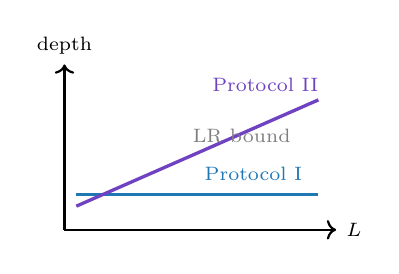
\begin{tikzpicture}[scale=0.75,
          ax/.style={->,thick},
          curve/.style={very thick}
        ]
        \draw[ax] (0,0)--(4.6,0) node[right,font=\scriptsize]{$L$};
        \draw[ax] (0,0)--(0,2.8) node[above,font=\scriptsize]{depth};
        \draw[curve,e0col] (0.2,0.6)--(4.3,0.6);
        \node[e0col,font=\scriptsize] at (3.2,0.95) {Protocol I};
        \draw[curve,midcol] (0.2,0.4)--(4.3,2.2);
        \node[midcol,font=\scriptsize] at (3.4,2.45) {Protocol II};
        \node[font=\scriptsize,gray] at (3.0,1.6) {LR bound};
      \end{tikzpicture}
    \end{column}
  \end{columns}
\end{frame}

% ============================================================
% Slide 4 — Motivation A: entanglement swapping
% ============================================================
\begin{frame}{Motivation A: entanglement swapping}
  \footnotesize
  \textbf{Primitive} (Żukowski–Zeilinger–Horne–Ekert, 1993):
  start with two Bell pairs $(A,B)$, $(C,D)$ — Bell-measure the middle pair $(B,C)$ —
  Pauli-correct $D$ based on the outcome — $A,D$ end up in $\ket{\Phi^+}$
  though they never interacted.

  \begin{center}
    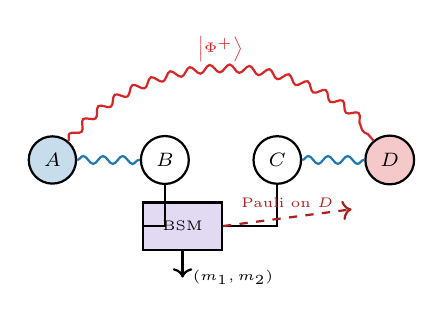
\begin{tikzpicture}[scale=0.85,
        qubit/.style={circle,draw,thick,minimum size=5mm,font=\scriptsize},
        bsm/.style={rectangle,draw,thick,fill=midcol!20,minimum height=6mm,minimum width=10mm,font=\tiny},
        ent/.style={decorate,decoration={snake,amplitude=0.5mm,segment length=2.5mm},thick,e0col},
        x=12mm
      ]
      \node[qubit,fill=e0col!25] (A) at (0,0) {$A$};
      \node[qubit] (B) at (1.4,0) {$B$};
      \node[qubit] (C) at (2.8,0) {$C$};
      \node[qubit,fill=e1col!25] (D) at (4.2,0) {$D$};
      \draw[ent] (A)--(B);
      \draw[ent] (C)--(D);
      \node[bsm,below=3mm of B.south east,anchor=north] (BSM) {BSM};
      \draw[thick] (B.south)|-(BSM.west);
      \draw[thick] (C.south)|-(BSM.east);
      \draw[->,thick] (BSM.south)--++(0,-0.4) node[right,font=\tiny]{$(m_1,m_2)$};
      \draw[->,dashed,thick,e1col!80!black] (BSM.east)--++(1.6,0.25)
        node[midway,above=0pt,font=\tiny]{Pauli on $D$};
      \draw[ent,e1col] (A) to[bend left=50] node[midway,above,font=\tiny]{$\ket{\Phi^+}$} (D);
    \end{tikzpicture}
  \end{center}

  \scriptsize
  Bäumer~\textit{et al.}, PRX Quantum~\textbf{5}, 030339 (2024) realised this
  primitive on 101 IBM qubits with constant-depth dynamic circuits.
\end{frame}

% ============================================================
% Slide 5 — Motivation B: GHZ-uncompute
% ============================================================
\begin{frame}{Motivation B: GHZ-uncompute (the unitary alternative)}
  \footnotesize
  \textbf{Idea.} If you cannot measure, build the entanglement everywhere
  and then carefully \emph{uncompute} what you don't want.
  \begin{enumerate}\setlength{\itemsep}{0.1em}
    \item Hadamard a central qubit, fan CNOTs outward
          $\Rightarrow$ GHZ $\frac{1}{\sqrt 2}(\ket{0\cdots0}+\ket{1\cdots1})$ across the top leg.
    \item Reverse the fan-out from the centre outward
          $\Rightarrow$ interior qubits return to $\ket{0}$; only the endpoints stay entangled.
  \end{enumerate}

  \begin{center}
    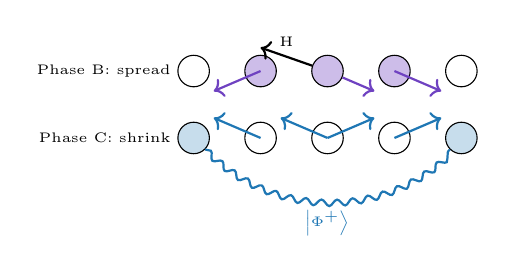
\begin{tikzpicture}[scale=0.85,
        q/.style={circle,draw,minimum size=4mm,inner sep=0pt,font=\tiny,fill=white},
        ghz/.style={q,fill=midcol!35},
        ent/.style={q,fill=e0col!25},
        arr/.style={->,thick},
        x=10mm
      ]
      \begin{scope}[shift={(0,0.9)}]
        \node[font=\tiny,anchor=east] at (-0.2,0) {Phase B: spread};
        \node[ghz] (m) at (2,0) {};
        \foreach \i in {1,3} {\node[ghz] at (\i,0) {};}
        \foreach \i in {0,4} {\node[q] at (\i,0) {};}
        \draw[arr] (m)--++(-1.0,0.35) node[midway,above,font=\tiny]{H};
        \draw[arr,midcol] (m)--++(0.7,-0.3);
        \draw[arr,midcol] (1,0)--++(-0.7,-0.3);
        \draw[arr,midcol] (3,0)--++(0.7,-0.3);
      \end{scope}
      \begin{scope}[shift={(0,-0.1)}]
        \node[font=\tiny,anchor=east] at (-0.2,0) {Phase C: shrink};
        \node[ent] (l) at (0,0) {};
        \foreach \i in {1,2,3} {\node[q] at (\i,0) {};}
        \node[ent] (r) at (4,0) {};
        \draw[arr,e0col] (2,0)--++(-0.7,0.3);
        \draw[arr,e0col] (1,0)--++(-0.7,0.3);
        \draw[arr,e0col] (2,0)--++(0.7,0.3);
        \draw[arr,e0col] (3,0)--++(0.7,0.3);
        \draw[e0col,decorate,decoration={snake,amplitude=0.4mm,segment length=2mm},thick]
          (l) to[bend right=45] node[midway,below,font=\tiny]{$\ket{\Phi^+}$} (r);
      \end{scope}
    \end{tikzpicture}
  \end{center}
  \scriptsize
  Cost: depth $L+2$, $2L-1$ CNOTs, \alert{zero measurements}. We call this
  \textbf{MOGU} = \emph{Middle-Out GHZ-Uncompute}.
\end{frame}

% ============================================================
% Slide 6 — Protocol I: overview circuit
% ============================================================
\begin{frame}{Protocol I — entanglement-swap with feed-forward}
  \footnotesize
  \textbf{Three layers, $O(1)$ depth:} (1)~three Bell pairs on alternating
  links; (2)~two parallel Bell-measurements on the inner pairs;
  (3)~classically-controlled Pauli correction on $e_1$.
  \begin{center}
    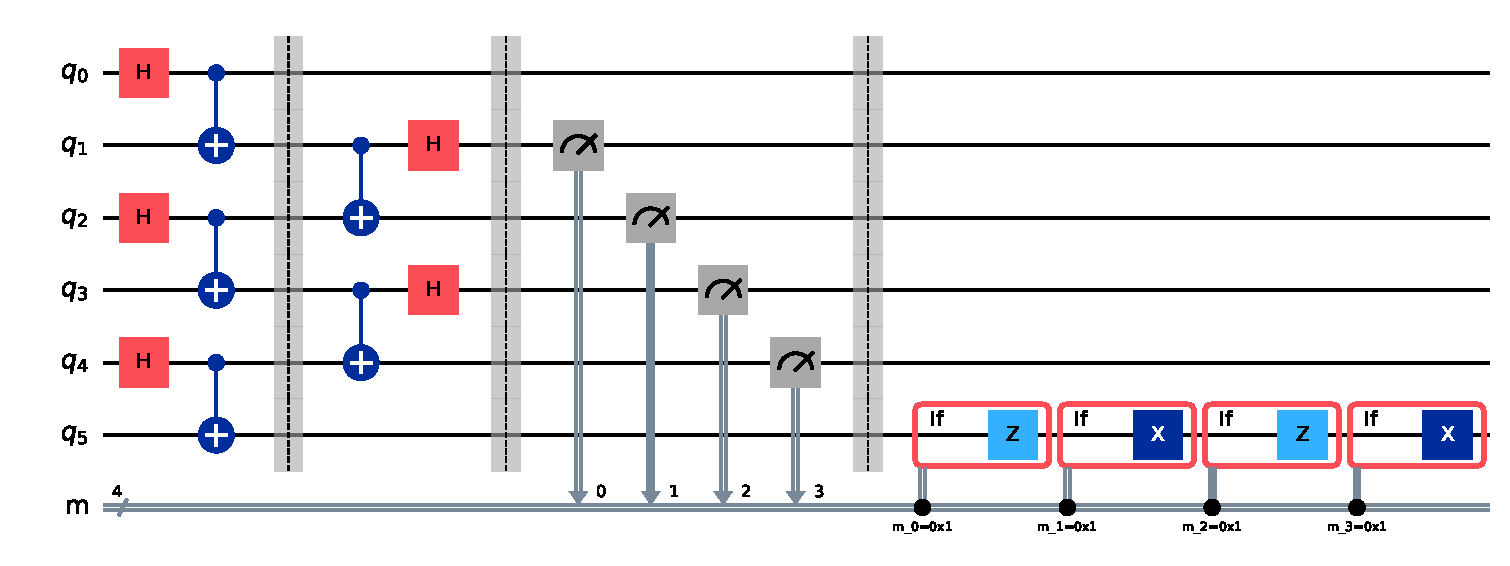
\includegraphics[width=0.95\textwidth]{../analysis/figures/circuit_swap_L5.pdf}
  \end{center}
\end{frame}

% ============================================================
% Slide 7 — Protocol I: equations
% ============================================================
\begin{frame}{Protocol I — the core math}
  After the Bell-measurement layer, the residual stabilisers on $(e_0,e_1)$
  reduce to
  \[
    \tilde P_{XX} = (-1)^{m_1+m_3}\,X_{e_0}X_{e_1},
    \qquad
    \tilde P_{ZZ} = (-1)^{m_2+m_4}\,Z_{e_0}Z_{e_1}.
  \]
  \pause
  Feed-forward Pauli correction on $e_1$:
  \[
    \boxed{\;X^{\,m_2\oplus m_4}\;Z^{\,m_1\oplus m_3}\;}
  \]
  collapses both signs to $+1$, so every measurement branch deterministically
  prepares $\ket{\Phi^+}_{e_0 e_1}$.
  \pause
  \medskip
  \begin{block}{Generalisation}
    \begin{itemize}
      \item Even $N$: induction on Bell-pair count $\Rightarrow$ depth $\leq 7$
            for all $L$.
      \item Odd $N$: a single GHZ-3 link at the tail handles the parity obstruction.
    \end{itemize}
  \end{block}

  \footnotesize
  \textbf{Resources.} $N{+}1$ or $N{+}2$ two-qubit gates, $N$ measurements,
  constant depth.
\end{frame}

% ============================================================
% Slide 8 — Protocol II: overview circuit
% ============================================================
\begin{frame}{Protocol II — MOGU (measurement-free)}
  \footnotesize
  \textbf{Three phases:} (1)~$H$ on middle qubit $q_{\lfloor L/2 \rfloor}$;
  (2)~\alert{spread} CNOTs fan out from middle to ends;
  (3)~\alert{shrink} reverse-fan-out disentangles every interior qubit, centre outward.
  \begin{center}
    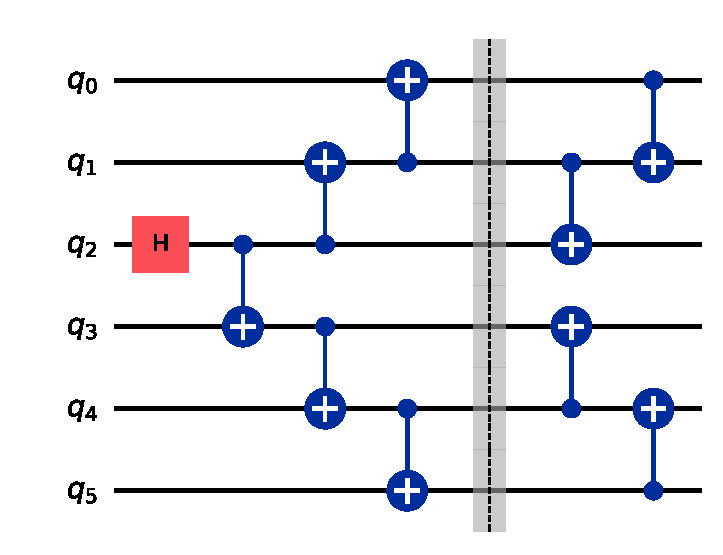
\includegraphics[height=0.62\textheight,keepaspectratio]{../analysis/figures/circuit_mogu_L5.pdf}
  \end{center}
\end{frame}

% ============================================================
% Slide 9 — Protocol II: equations + parallel remark
% ============================================================
\begin{frame}{Protocol II — core formulas}
  \textbf{Sequential schedule.}
  \[
    \text{depth} = L+2,\quad
    \text{2Q gates} = 2L-1,\quad
    \text{measurements} = 0.
  \]
  \pause
  \textbf{Stabiliser sketch.} After Phase~B the state is the standard $(L{+}1)$-qubit
  GHZ. Phase~C peels off each interior $Z_i$ generator, leaving
  \[
    \langle X_{e_0}X_{e_1},\; Z_{e_0}Z_{e_1},\; Z_1,\dots,Z_{L-1}\rangle
    \;=\; \text{stab}\bigl(\ket{\Phi^+}_{e_0 e_1}\otimes\ket{0}^{\otimes L-1}\bigr).
  \]
  \pause
  \textbf{Parallel schedule} (documentation-only, not in the verified code):
  if we interleave Phase~C with the still-in-flight Phase~B, the depth drops to
  \[
    d_{\parallel}(L) \;\approx\;
      \begin{cases}
        \min(L+2,\; \lceil L/2\rceil + 4) & L\ \text{even},\\
        \min(L+1,\; \lceil L/2\rceil + 3) & L\ \text{odd}.
      \end{cases}
  \]
  \footnotesize\emph{$\approx 2\times$ depth reduction at large $L$ — free constant-factor win.}
\end{frame}

% ============================================================
% Slide 10 — Benchmark scaling
% ============================================================
\begin{frame}{Benchmark: resources vs $L$}
  \begin{center}
    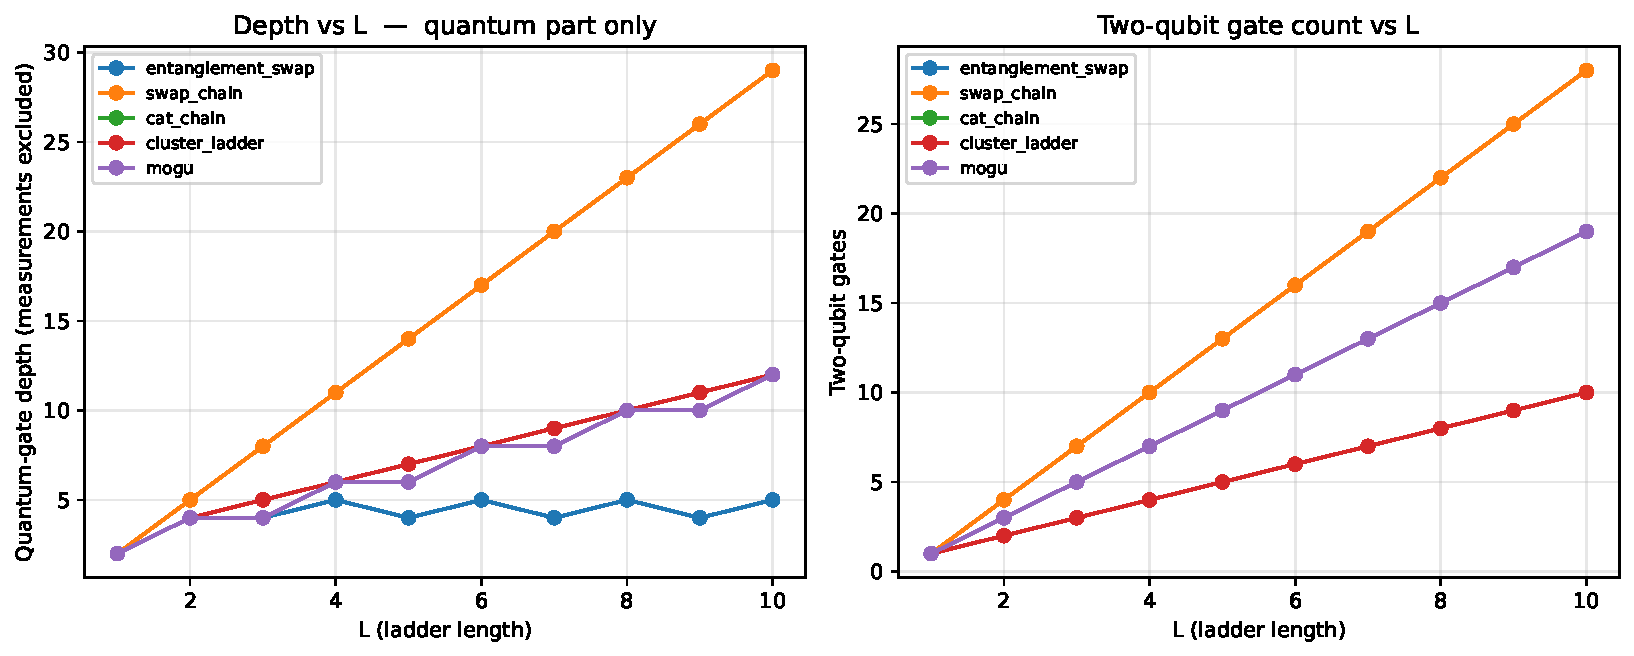
\includegraphics[width=0.96\textwidth]{../analysis/figures/scaling_quantum.pdf}
  \end{center}
  \vspace{-0.3em}
  \footnotesize
  \textbf{What you see.} Protocol~I (\textcolor{e0col}{blue}) is the
  \alert{only depth-$O(1)$ curve} — its quantum part stays at $\leq 5$ layers
  for every $L$. Measurements and feed-forward Paulis are excluded from this
  count (they execute in classical real time). MOGU is linear with the smallest
  slope among the unitary protocols; SWAP-chain dominates both axes.
\end{frame}

% ============================================================
% Slide 11 — Benchmark noise
% ============================================================
\begin{frame}{Benchmark: Bell fidelity under depolarising noise}
  \begin{columns}[T,onlytextwidth]
    \begin{column}{0.62\textwidth}
      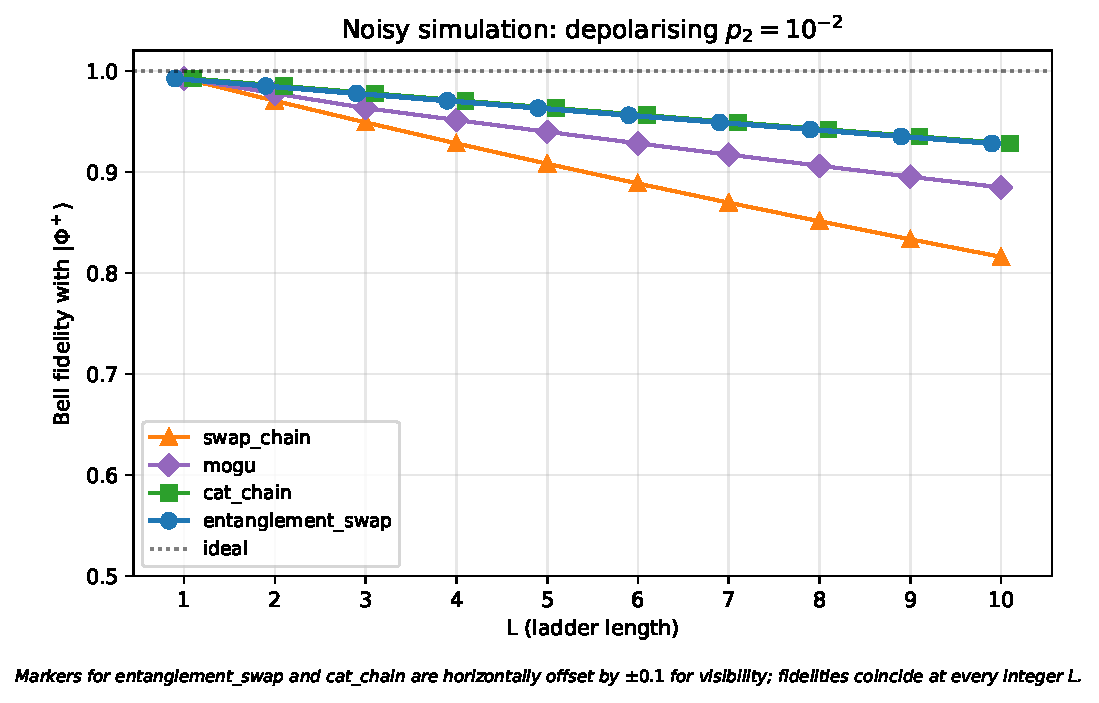
\includegraphics[width=\linewidth]{../analysis/figures/noise_slides.pdf}
    \end{column}
    \begin{column}{0.38\textwidth}
      \footnotesize
      Symmetric two-qubit depolarising error $p_2=10^{-2}$ on every CNOT.
      \medskip

      \textbf{At $L=10$:}
      \begin{itemize}\setlength{\itemsep}{0.15em}
        \item Protocol~I: \alert{$0.928$}
        \item cat\_chain: $0.928$ \;{\scriptsize(same 2Q-gate count)}
        \item MOGU: $0.885$
        \item swap\_chain: $0.816$
      \end{itemize}

      \medskip
      Protocol~I (\textbf{$\bullet$}) and cat\_chain (\textbf{$\blacksquare$})
      give \emph{identical} fidelities at every $L$ — both incur $\approx N$
      noisy CNOTs touching $(e_0, e_1)$. The markers are jittered by
      $\pm 0.1$ in $L$ purely for visibility.
    \end{column}
  \end{columns}
\end{frame}

% ============================================================
% Slide 12 — When to use which
% ============================================================
\begin{frame}{When to prefer which protocol}
  \centering\footnotesize
  \begin{tabular}{lll}
    \toprule
    \textbf{Hardware regime} & \textbf{Best choice} & \textbf{Why} \\
    \midrule
    Mid-circuit measurement + feed-forward & Protocol~I & $O(1)$ depth \\
    Unitary-only                           & MOGU       & saturates LR bound \\
    Small $L$, deep noise budget           & cat\_chain & fewest gates per endpoint \\
    \bottomrule
  \end{tabular}

  \vspace{0.6em}
  \begin{itemize}\footnotesize\setlength{\itemsep}{0.15em}
    \item Both protocols verified to fidelity $>1-10^{-9}$ via \texttt{stim}
          Clifford and Qiskit \texttt{Statevector} for $L\le 10$;
          spot checks at $L\in\{20,30,50\}$.
    \item \textbf{132 automated tests}, all passing.
    \item Single codebase under \texttt{analysis/}.
  \end{itemize}
\end{frame}

% ============================================================
% Slide 13 — Thanks / references
% ============================================================
\begin{frame}[allowframebreaks]{References \& summary}
  \textbf{Take-home.}
  \begin{itemize}
    \item Two protocols, one ladder, complementary hardware assumptions.
    \item Protocol~I: $O(1)$ depth, classical feed-forward.
    \item Protocol~II (MOGU): $L+2$ depth, measurement-free, depth-optimal for unitary 1D.
  \end{itemize}

  \medskip
  \textbf{Key references.}
  \begin{itemize}\footnotesize
    \item Żukowski, Zeilinger, Horne, Ekert,
          \emph{Phys. Rev. Lett.}~\textbf{71}, 4287 (1993) — entanglement swapping primitive.
    \item Briegel, Dür, Cirac, Zoller,
          \emph{Phys. Rev. Lett.}~\textbf{81}, 5932 (1998) — quantum repeater.
    \item Bäumer~\textit{et al.},
          \emph{PRX Quantum}~\textbf{5}, 030339 (2024), arXiv:2308.13065 —
          long-range CNOT teleportation on 101 IBM qubits.
    \item Song~\textit{et al.},
          \emph{Phys. Rev. Applied}~\textbf{24}, 024068 (2025), arXiv:2409.06989 —
          constant-depth fan-out with feedforward.
  \end{itemize}

  \medskip
  \centering\Large Thank you. \\[0.3em]
  \small Questions?
\end{frame}

\end{document}
